\documentclass{standalone}

%maths
\usepackage{tikz}
\usepackage{scalerel}
\usepackage{pict2e}
\usepackage{tkz-euclide}
\usetikzlibrary{calc}
\usetikzlibrary{patterns,arrows.meta}
\usetikzlibrary{shadows}
\usetikzlibrary{external}

%pgfplot

\usepackage{pgfplots}
\pgfplotsset{compat=newest}
\usepgfplotslibrary{statistics}
\usepgfplotslibrary{fillbetween}

%colours
\usepackage{xcolor}

\begin{document}
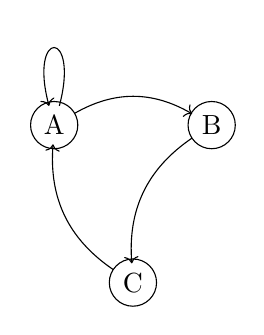
\begin{tikzpicture}


\node (A) at (0,0) {A};
\node (B) at (2,0) {B};
\node (C) at (1,-2) {C};

\draw (0,0) circle (0.3);
\draw (2,0) circle (0.3);
\draw (1,-2) circle (0.3);

\draw[->, bend left] (A) to (B); 
\draw[->, bend right] (B) to (C); 
\draw[->, bend left] (C) to (A);

\draw[<-, loop above, looseness=20] (A) to (A);





\end{tikzpicture}



\end{document}

